\section{Guidance - Navigation - Control}

\begin{frame}{Guidance - Navigation - Control}
	\framesubtitle{GNC overview}
	In the previous section, we introduce the modeling and mathematical model to describe the dynamics behavior. In the following steps, the control techniques, which include guidance, navigation and motion control, for a specific underwater vehicle (in general, consider the ocean vehicle).  The theory and cases studies are organized as three independent part:
	\begin{itemize}
		\item \textbf{G -  Guidance Systems}: Systems for automatically guiding the path of a marine craft, usually without direct or continuous human control.
		\item \textbf{N -  Navigation Systems}: Systems for determination of the craft’s position/attitude, velocity and acceleration.
		\item \textbf{C - Control Systems}: PID design methods for automatic control of position/attitude,
		velocity and acceleration. This involves control systems for stabilization, trajectory-tracking and path following control of marine craft.
	\end{itemize}
\end{frame}




% =========================================
% =========================================




\begin{frame}{Guidance - Navigation - Control}
	\framesubtitle{GNC overview}
	\begin{tikzpicture}[remember picture,overlay]
		% \node[fill=blue!30, text=white, font=\large, rounded corners] 
		\node at (current page.north east) [xshift=-6cm, yshift=-3cm] 
		{\includegraphics[width=0.7\linewidth]{img/GNC.png}};
	\end{tikzpicture}
	
	\begin{tikzpicture}[remember picture,overlay]
		% \node[fill=blue!30, text=white, font=\large, rounded corners] 
		\node at (current page.north east) [xshift=-6cm, yshift=-7cm] 
		{\includegraphics[width=0.7\linewidth]{img/GNC1.png}};
	\end{tikzpicture}
	
\end{frame}






% =========================================
% =========================================




\begin{frame}{Guidance - Navigation - Control}
	\framesubtitle{Setpoint regulation, trajectory-tracking control and path-following control}
	\textbf{Setpoint Regulation:} The most basic guidance system is {\color{red}a constant input or setpoint provided by a human operator}. The corresponding controller will then be a regulator. Examples of setpoint regulation are constant depth, trim, heel and speed control. It could also be regulation to zero, which is commonly required in roll and pitch for instance.
	
	\textbf{Trajectory-Tracking Control:} The position and velocity of the marine craft should {\color{red}track desired time varying position and velocity reference signals}. The corresponding feedback controller is a trajectory tracking controller. Tracking control can be used for course-changing maneuvers, speed-changing and attitude control. An advanced guidance system computes optimal time-varying trajectories from a dynamic model for a predefined control objective. If a constant setpoint is used as input to a low-pass filter (reference model) in an open-loop guidance system, the outputs of the filter will be smooth time-varying reference trajectories for position, velocity and acceleration (PVA).
	
	\textbf{Path-Following Control:} This is to {\color{red} follow a predefined path independent of time} (no temporal constraints). Moreover, no restrictions are placed on the temporal propagation along the path. This is typical for ships in transit between continents or underwater vehicles used to map the seabed.
\end{frame}



% =========================================
% =========================================




\begin{frame}{Guidance - Navigation - Control}
	\framesubtitle{Guidance - Target tracking}
	\begin{tikzpicture}[remember picture,overlay]
		% \node[fill=blue!30, text=white, font=\large, rounded corners] 
		\node at (current page.north east) [xshift=-6cm, yshift=-3.5cm] 
		{\includegraphics[width=0.8\linewidth]{img/Guidance.png}};
	\end{tikzpicture}
	
	\vspace{3cm}
	Several guidance strategies
	\begin{itemize}
		\item Line-of-Sight Guidance (LOS)
		\item Pure Pursuit Guidance (PP)
		\item Constant Bearing Guidance (CB)
		\item ...
	\end{itemize}
\end{frame}


% =========================================
% =========================================

\begin{frame}{Guidance - Navigation - Control}
	\framesubtitle{Guidance - Trajectory tracking}
	\begin{tikzpicture}[remember picture,overlay]
		% \node[fill=blue!30, text=white, font=\large, rounded corners] 
		\node at (current page.north east) [xshift=-6cm, yshift=-3.5cm] 
		{\includegraphics[width=0.8\linewidth]{img/Guidance1.png}};
	\end{tikzpicture}
	
	\vspace{3cm}
	
	The easiest approach is that the desired trajectory can be computed using reference models generated by 	low-pass filters
	\begin{align}
		\dfrac{x_d}{r}(s) = h_{lp}(s) = \dfrac{\omega^2}{s^2 + 2\xi\omega s + \omega^2}
	\end{align}
	where $r(s)$ is set up by operator and $x_d(s)$ is the controller input.
\end{frame}


% =========================================
% =========================================

\begin{frame}{Guidance - Navigation - Control}
	\framesubtitle{Guidance - Trajectory tracking}
	The second one is that we consider the simulation model to generate the trajectory. For instance, a dynamic model could be chosen as
	\begin{align}
		\dot{\eta}_d = J(\eta)\nu_d \\
		M\dot{\nu}_d + N\nu_d + g(\nu_d) = \tau
	\end{align}
	The smooth trajectory could be generated by simulating the above dynamic model with a certain controller, such as PD control. To explain,
	\begin{align}
		\tau = g(\eta_d) - J^{-1}(\eta_d)(K_p(\eta_d - \eta_{ref}) + Kd\dot{\eta}_d)
	\end{align}
\end{frame}



% =========================================
% =========================================

\begin{frame}{Guidance - Navigation - Control}
	\framesubtitle{Guidance - Trajectory tracking}
	The vehicles' trajectory could be generated by optimization problems. The easiest approach method for this problem by consider a cost function of power, or time, and the purpose is to minimize this cost function. That mean,
	\begin{align}
		x_d* = \text{argmin}_{x_d}\Big(f(x, t)\Big) \\
		s.t. \quad x_d \in \mathcal{X} 
	\end{align}
	For examples, by considering the discrete model of vehicles, the optimization problem could be expressed in detail as follows 
	\begin{align}
		x_d^* = \text{argmin}_{x_d}\sum x_d(k)^\top Q x_d(k)\\
		or\\
		x_d^* = \text{argmin}_{x_d} t
	\end{align}
	with constraint $x_d(k+1) = f(x_d(k), u(k))$ and $Q = Q^\top > 0$
\end{frame}


% =========================================
% =========================================

\begin{frame}{Guidance - Navigation - Control}
	\framesubtitle{Guidance - Path following}
	Path generation using straight lines and Circular Arcs
	
	\textit{ The shortest path (minimum time) between two configurations $(x, y, \psi)$ of a craft moving at constant speed U is a path formed by straight lines and circular arc segments.}
	
	\vspace{5cm}
	
	\begin{tikzpicture}[remember picture,overlay]
		% \node[fill=blue!30, text=white, font=\large, rounded corners] 
		\node at (current page.north east) [xshift=-3cm, yshift=-6cm] 
		{\includegraphics[width=0.5\linewidth]{img/path_gen.png}};
	\end{tikzpicture}
	
	\begin{tikzpicture}[remember picture,overlay]
		% \node[fill=blue!30, text=white, font=\large, rounded corners] 
		\node at (current page.north east) [xshift=-9.5cm, yshift=-6cm] 
		{\includegraphics[width=0.5\linewidth]{img/path_gen1.png}};
	\end{tikzpicture}
	
\end{frame}


% =========================================
% =========================================

\begin{frame}{Guidance - Navigation - Control}
	\framesubtitle{Guidance - Path following}
	First of all, we consider \textbf{a Straight-line path} and introduce two different guidance principles, which could be used to steer along the LOS vector:
	\begin{itemize}
		\item Enclosure-based steering $\to$ find $(x_{los}, y_{los})$ base on a a circle with radius $R>0$ enclosuring $(x, y)$
		\item Lookahead-based steering $\to$ steering law could be easy to modify
	\end{itemize}
	
	\vspace{5cm}
	
	
	
	\begin{tikzpicture}[remember picture,overlay]
		% \node[fill=blue!30, text=white, font=\large, rounded corners] 
		\node at (current page.north east) [xshift=-9.5cm, yshift=-6.5cm] 
		{\includegraphics[width=0.5\linewidth]{img/path follow.png}};
	\end{tikzpicture}
	
	
	\begin{tikzpicture}[remember picture,overlay]
		% \node[fill=blue!30, text=white, font=\large, rounded corners] 
		\node at (current page.north east) [xshift=-3.5cm, yshift=-6.5cm] 
		{\includegraphics[width=0.5\linewidth]{img/path follow1.png}};
	\end{tikzpicture}
	
\end{frame}



% =========================================
% =========================================

\begin{frame}{Guidance - Navigation - Control}
	\framesubtitle{Guidance - Path following}
	
	
	\begin{tikzpicture}[remember picture,overlay]
		% \node[fill=blue!30, text=white, font=\large, rounded corners] 
		\node at (current page.north east) [xshift=-7cm, yshift=-3.5cm] 
		{\includegraphics[width=0.8\linewidth]{img/path follow2.png}};
	\end{tikzpicture}
	
	\vspace{3cm}
	
	\begin{itemize}
		\item Enclosure-based steering law $\to$ $\psi_d = atan2(y_{los} - y, x_{los} - x)$
		\item Lookahead-based steering law $\to$ $\psi_d = \chi_d - \beta = \alpha_k + arctan(-\text{PID}(e)) - \beta$
	\end{itemize}
	\textbf{Repeat again:} $\beta$ is the sideslip angle, which calculated by $\beta = arcsin(v/U)$
	
\end{frame}




% =========================================
% =========================================

\begin{frame}{Guidance - Navigation - Control}
	\framesubtitle{Guidance - Path following}
	In the following, \textbf{Path-Following for Curved Paths} is introduced.
	
	MATLAB provide different methods for interpolation. For example, three methods for path generation are the cubic spline interpolant (\texttt{spline.m}), piecewise cubic Hermite interpolanting polynomial (\texttt{pchip.m}) and modified Akima piecewise cubic Hermite interpolation (\texttt{makima.m})
	
	\vspace{4cm}
	
	
	\begin{tikzpicture}[remember picture,overlay]
		% \node[fill=blue!30, text=white, font=\large, rounded corners] 
		\node at (current page.north east) [xshift=-9.5cm, yshift=-6.5cm] 
		{\includegraphics[width=0.5\linewidth]{img/path follow4.png}};
	\end{tikzpicture}
	
	
	\begin{tikzpicture}[remember picture,overlay]
		% \node[fill=blue!30, text=white, font=\large, rounded corners] 
		\node at (current page.north east) [xshift=-3.5cm, yshift=-6.5cm] 
		{\includegraphics[width=0.5\linewidth]{img/path follow3.png}};
	\end{tikzpicture}
\end{frame}






% =========================================
% =========================================


\begin{frame}{Guidance - Navigation - Control}
	\framesubtitle{Guidance - Path following}
	In other approach, which is called cubic polynomials, we consider a parametrized path as follows
	\begin{align}
		x_d(\varpi) = \sum\limits_{i = 0}^3 a_i\varpi^i; \qquad y_d(\varpi) = \sum\limits_{i = 0}^3 b_i\varpi^i
	\end{align}
	Then, the above constraints must be satisfied
	\begin{align}
		x_d(\varpi_{k-1}) = x_{k - 1}, \quad x_d(\varpi_{k}) = x_{k},\\
		\lim\limits_{\varpi \to \varpi_{k}^{-}} \dfrac{d\,x_d(\varpi_{k})}{d\,\varpi_{k}} = \lim\limits_{\varpi \to \varpi_{k}^{+}} \dfrac{d\,x_d(\varpi_{k})}{d\,\varpi_{k}}\\
		\lim\limits_{\varpi \to \varpi_{k}^{-}} \dfrac{d^2\,x_d(\varpi_{k})}{(d\,\varpi_{k})^2} = \lim\limits_{\varpi \to \varpi_{k}^{+}} \dfrac{d^2\,x_d(\varpi_{k})}{(d\,\varpi_{k})^2}\\
		\dfrac{d\,x_d(\varpi_{k})}{d\,\varpi_{k}}(\varpi_0) = const, \quad \dfrac{d\,x_d(\varpi_{k})}{d\,\varpi_{k}}(\varpi_n) = const\\
		OR \quad \Bigg(\dfrac{d^2\,x_d(\varpi_{k})}{(d\,\varpi_{k})^2}(\varpi_0) = const, \quad \dfrac{d^2\,x_d(\varpi_{k})}{(d\,\varpi_{k})^2}(\varpi_n) = const\Bigg)
	\end{align}
\end{frame}





% =========================================
% =========================================

\begin{frame}{Guidance - Navigation - Control}
	\framesubtitle{Guidance - Path following}
	\begin{tikzpicture}[remember picture,overlay]
		% \node[fill=blue!30, text=white, font=\large, rounded corners] 
		\node at (current page.north east) [xshift=-6.5cm, yshift=-5cm] 
		{\includegraphics[width=\linewidth]{img/path follow5.png}};
	\end{tikzpicture}
	
\end{frame}




% =========================================
% =========================================

\begin{frame}{Guidance - Navigation - Control}
	\framesubtitle{Guidance - Path following}
	\textbf{Transformation of Path to Reference Trajectories using Desired Speed Profiles}
	
	\begin{align}
		\dot{\varpi}(t) = \dfrac{U_d(t)}{\sqrt{\dfrac{d\,x_d(\varpi_{k})}{d\,\varpi_{k}}(\varpi)^2 + \dfrac{d\,x_d(\varpi_{k})}{d\,\varpi_{k}}(\varpi)^2}}\\
		T\dot{U}_d(t) + U_d(t) = U_{ref}
	\end{align}
	
	
\end{frame}



% =========================================
% =========================================

\begin{frame}{Guidance - Navigation - Control}
	\framesubtitle{Guidance - Path following}
	In another view, the cubic polynomials approach could be formed by the \textbf{Nonlinear Constrained Optimization Problem}. Firstly, the constraint of the cubic polynomials approach could be represented by the the linear form
	\begin{align}
		y = A(t_k, t_{k + 1})x
	\end{align}
	where $x$ is the vector of polynomial coefficients, and $y$, $A$ are the derived constraints vector and matrix. Then, the optimization problem is formed
	\begin{align}
		\text{minimize} \Big[\Big(A(t_k, t_{k + 1})x - y\Big)^\top\Big(A(t_k, t_{k + 1})x - y\Big)\Big]
	\end{align}
	with the constraint of velocities and accelerations.
\end{frame}




% =========================================
% =========================================

\begin{frame}{Guidance - Navigation - Control}
	\framesubtitle{Guidance - Path following}
	
	\begin{columns}[onlytextwidth]
		\column{.5\textwidth}
		The solution to the problem of path-following proposed here builds on the following intuitive explanation a simple path-following controller should compute 
		
		(i) the distance between the vehicle’s center of mass $Q$ and a point $P$, and 
		
		(ii) the angle between the vehicle’s total velocity vector $v_t$ and the tangent to the path at $P$, and reduce both to zero. This motivates the development of the `kinematic' model of the vehicle in terms of a Serret–Frenet frame $\{F\}$ that moves along the path; $\{F\}$ plays the role of the body axis of a ‘virtual target vehicle’ that should be tracked by the `real vehicle'.
		\column{.5\textwidth}
	\end{columns}
	
	
	\begin{tikzpicture}[remember picture,overlay]
		% \node[fill=blue!30, text=white, font=\large, rounded corners] 
		\node at (current page.north east) [xshift=-3cm, yshift=-5cm] 
		{\includegraphics[width=0.5\linewidth]{img/path follow6.png}};
	\end{tikzpicture}
	
\end{frame}




% =========================================
% =========================================

\begin{frame}{Guidance - Navigation - Control}
	\framesubtitle{Guidance - Path following}
	
	\begin{columns}[onlytextwidth]
		\column{.5\textwidth}
		\small
		\begin{align}
			\dot{s}_1 &= -\dot{s}(1 - c_c y_1) + v_t \cos\psi, \\
			\dot{y}_1 &= -c_c \dot{s}_1 + v_t \sin\psi, \\
			\dot{\psi} &= r + \dot{\beta}- c_c \dot{s}.
		\end{align}
		
		Assuming we have a precise estimation of the function $\mu(s)$, and given $s$, we compute
		\begin{align}
			x_s(\mu) = \sum_{i=1}^n a_i \mu^i, \quad y_s(\mu) = \sum_{i=1}^n b_i \mu^i,\\
			\psi_F(s) = \arctan\left(\frac{(y_s)'}{(x_s)'}\right), \\
			c_c(s) = \frac{\partial \psi_F(s)}{\partial \mu} \frac{d\mu}{ds}, \\
			\frac{\partial c_c(s)}{\partial s} = \frac{\partial c_c(s)}{\partial \mu} \frac{d\mu}{ds}, \\
			(x_s)' = \frac{dx_s}{d\mu}, \quad (y_s)' = \frac{dy_s}{d\mu}\\
			\frac{d\mu}{ds} = \frac{1}{\sqrt{[(x_s)']^2 + [(y_s)']^2}}.
		\end{align}
		\column{.5\textwidth}
	\end{columns}
	
	
	\begin{tikzpicture}[remember picture,overlay]
		% \node[fill=blue!30, text=white, font=\large, rounded corners] 
		\node at (current page.north east) [xshift=-3.2cm, yshift=-5cm] 
		{\includegraphics[width=0.5\linewidth]{img/path follow7.png}};
	\end{tikzpicture}
	
\end{frame}






% =========================================
% =========================================

\begin{frame}{Guidance - Navigation - Control}
	\framesubtitle{Navigation}
	\begin{tikzpicture}[remember picture,overlay]
		% \node[fill=blue!30, text=white, font=\large, rounded corners] 
		\node at (current page.north east) [xshift=-6cm, yshift=-3cm] 
		{\includegraphics[width=0.7\linewidth]{img/navigation.png}};
	\end{tikzpicture}
	
	\begin{tikzpicture}[remember picture,overlay]
		% \node[fill=blue!30, text=white, font=\large, rounded corners] 
		\node at (current page.north east) [xshift=-6cm, yshift=-6.5cm] 
		{\includegraphics[width=0.6\linewidth]{img/navigation1.png}};
	\end{tikzpicture}
\end{frame}




% =========================================
% =========================================

\begin{frame}{Guidance - Navigation - Control}
	\framesubtitle{Navigation - Low-Pass and Notch filtering}
	\textbf{Low-Pass filtering}: $\omega_b \ll \omega_e$, 
	\begin{align}
		\hat{y}(s) = h_{lp}(s)y(s)
	\end{align}
	where $h_{lp}(s)$ could be chosen as first-order low-pass filter, $h_{lp}(s) = \dfrac{1}{1 + T_fs}$ or the higher-order low-pass filter by using Butterworth filter, $h_{lf}(s) = \dfrac{1}{p(s)}$, with $p(s)p(-s) = 1 + (s/j\omega_f)^{2n}$
	
	\textbf{Cascade Low-Pass and Notch filtering}: 
	\begin{align}
		\hat{y}(s) = h_{lp}(s)h_{n}(s)y(s)
	\end{align}
	with 
	\begin{align}
		h_n(s) = \dfrac{s^2 + 2\xi\omega_ns + \omega_n^2}{(s + \omega_n)^2}; \quad OR \quad h_n(s) = \prod_{i=1}^{3}\dfrac{s^2 + 2\xi\omega_is + \omega_i^2}{(s + \omega_i)^2}
	\end{align}
	
\end{frame}



% =========================================
% =========================================

\begin{frame}{Guidance - Navigation - Control}
	\framesubtitle{Navigation - Observer}
	Consider the linear time-invariant (LTI) system, 
	\begin{align}
		\dot{x} = Ax + Bu\\
		y = Cx
	\end{align}
	and consider its dual system
	\begin{align}
		\dot{\tilde{x}} = A^\top\tilde{x} + C^\top\tilde{u}\\
		\tilde{y} = B^\top\tilde{x}
	\end{align}
	\textbf{Luenberger observer}: coud be designed as \textbf{pole placement control design} for the dual system.

	\textbf{Kalman observer}: coud be designed as \textbf{LQR control design} for the dual system.
	
	Both of above-mentioned observers follow the bellow structure
	\begin{align}
		\dot{z} = Az + Bu + L(y - Cz)
	\end{align}
	with $L$ is observer gain.
	
\end{frame}


% =========================================
% =========================================

\begin{frame}{Guidance - Navigation - Control}
	\framesubtitle{Navigation - Observer}
	In other way, the advance observers that we could approach
	\begin{itemize}
		\item Extended Kalman Filter
		\item High-gain observer
		\item Sliding Mode Observer
		\item Extended State observer
		\item Fixed- and Finite-time observer
		\item ...
	\end{itemize}
	
\end{frame}

% =========================================
% =========================================

\begin{frame}{Guidance - Navigation - Control}
	\framesubtitle{Control - PID control}
	\begin{tikzpicture}[remember picture,overlay]
		% \node[fill=blue!30, text=white, font=\large, rounded corners] 
		\node at (current page.north east) [xshift=-6cm, yshift=-4cm] 
		{\includegraphics[width=0.7\linewidth]{img/feedback control.png}};
	\end{tikzpicture}
	
	
	\vspace{4.5cm}
	
	Closed-loop feedback system - PID control approach
	\begin{align}
		\tau_{PID} = -K_pe - K_d\dot{e} - K_i\int\limits_{0}^{t}e(\tau)d\tau
	\end{align}
\end{frame}



% =========================================
% =========================================



\begin{frame}{Guidance - Navigation - Control}
	\framesubtitle{Linear control approach}
	In the below section, we approach the control problem of linear system by Linear control technique.
	
	First of all, consider the linearization algorithm for nonlinear system, 
	
	\vspace{1cm}
	
	\begin{minipage}{.5\textwidth}
		\hspace{0cm}
		Assume that, the linear function at $B$ is
		\begin{align}
			y &= a_Bx + b_B \\
			&\approx F(x) \Big|_{x \in \Delta_{x_B}}
		\end{align}
		where $a_B$ is the coefficient of first degree, easy to determine
		\begin{align}
			a_B = \dfrac{\partial F(x)}{\partial x}\Bigg|_{x = x_B}
		\end{align}
		and $b_B$ is the bias.
	\end{minipage}%
	\begin{minipage}{.5\textwidth}
		\hspace{+0.25cm}
		\centering
		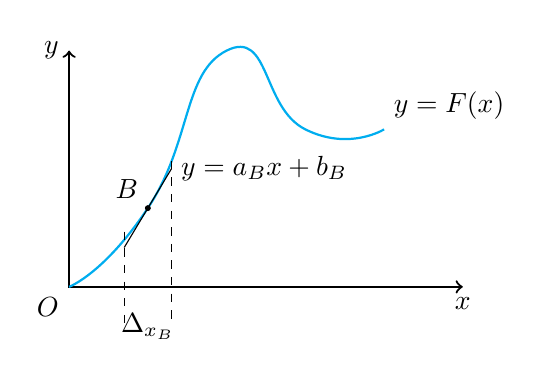
\begin{tikzpicture}
			% \draw (0, 0) grid (5, 5);
			\draw [<->, thick] (5, 0) node[below]{$x$} -- (0, 0) node[below left]{$O$} -- (0, 3) node[left]{$y$};
			\draw [cyan, thick] plot [smooth, tension=1] coordinates { (0,0) (1,1) (2,3) (3,2) (4,2)};
			\draw (4, 2) node[above right] {$y = F(x)$};
			\coordinate (A) at (3, 2);
			\coordinate (B) at (1, 1);
			\draw [fill = black] (B) node[above left] {$B$} circle (0.03);
			
			\draw (0.7, 0.5) -- (1.3, 1.5) node [right] {$y = a_Bx + b_B$};
			\draw [dashed] (0.7, 0.7) -- (0.7, -0.5);
			\draw [dashed] (1.3, 1.6) -- (1.3, -0.5);
			\draw (1, -0.5) node {$\Delta_{x_B}$};
			
		\end{tikzpicture}
	\end{minipage}
\end{frame}

% =========================================
% =========================================


\begin{frame}{Guidance - Navigation - Control}
	\framesubtitle{Linear control approach}
	Consider a general system, which found in the above
	\begin{align}
		\Dot{{x}} = f({x}) + g({x})\tau = F({x}, \tau)
	\end{align}
	$\to$ Let's approximate it to the linear original difference equation (ODE)
	\begin{align}
		\Dot{{x}} = {A}{x} + {B}\tau
	\end{align}
	where, the state-space matrices are defined as
	\begin{align}
		{A} = \dfrac{\partial F({x}, \tau)}{\partial {x}}\Bigg|_{{x} = {x}_e,\tau = \tau_e} \\
		{B} = \dfrac{\partial F({x}, \tau)}{\partial \tau}\Bigg|_{{x} = {x}_e, \tau = \tau_e}
	\end{align}
\end{frame}

% =========================================
% =========================================





\begin{frame}{Guidance - Navigation - Control}
	\framesubtitle{State-Space-based Linear control approach}
	{\color{red} In the following step, we propose a linear control technique - pole placement control.}
	
	\vspace{0.5cm}
	
	First, consider the state-space model, described as follows
	\begin{align}
		\Dot{{x}} = {A}{x} + {B}\tau \label{eqn: system}
	\end{align}
	As mention above, the control signal is 
	\begin{align}
		\tau = h({x})
	\end{align}
	such as, the system in (\ref{eqn: system}) is stable.\\ 
	For simplify the control signal, we assume that, the control law is a gain of state variables
	\begin{align}
		\tau = h({x}) = -{K}{x}
	\end{align}
	{\color{red} This is the most simplify of control law!}
\end{frame}



% =========================================
% =========================================



\begin{frame}{Guidance - Navigation - Control}
	\framesubtitle{State-Space-based Linear control approach}
	With the control signal defined as $\tau = h({x}) = -{K}{x}$, the close-loop system becomes
	\begin{align}
		\Dot{{x}} &= {A}{x} - {B}{K}{x} \\
		& = ({A} - {B}{K}){x}
	\end{align}
	Let $\Tilde{{A}} = {A} - {B}{K}$. This ODE exist the solution as
	\begin{align}
		{x} = \text{e}^{\Tilde{{A}}t} = \sum\limits_{i = 0}^{\infty}\dfrac{\Tilde{{A}}^it^i}{i!} = {P}^{-1}\Big(\sum\limits_{i = 0}^{\infty}\dfrac{{L}^it^i}{i!} \Big) {P}=  {P}^{-1}\text{e}^{{L}t} {P}
	\end{align}
	where 
	\begin{align}
		{L} = diag(\lambda_1, \lambda_2, ..., \lambda_i)
	\end{align}
	$\lambda_i$ are the eigenvalue of $\Tilde{{A}}$ with eigenvector ${P}_i$ and
	\begin{align}
		{P} = \begin{bmatrix}
			{P}_1^\top & {P}_2^\top & ... & {P}_i^\top
		\end{bmatrix}^\top
	\end{align}\\
	{\color{red} Find ${K}$ such as $\lim_{t \to \infty}{x} = 0$ that mean Find ${K}$ such as ${L} < 0$}
\end{frame}






% =========================================
% =========================================



\begin{frame}{Guidance - Navigation - Control}
	\framesubtitle{State-Space-based Linear control approach}
	{\color{red} Similarly, by considering a optimization problem, Linear Quadratic Regulator is constructed.}
	
	
	First of all, consider linear time-invariant system
	\begin{align}
		\dfrac{d}{dt}{x} = {A}{x} + {B}u
	\end{align}
	and control signal for this system
	\begin{align}
		{u} = {\omega} - G{x}
	\end{align}
	The LQR controller is a state feedback controller, with the control signal $u$ found to be satisfied
	\begin{align}
		J = \dfrac{1}{2}\int\limits_{0}^\infty\Big({x}^T{Q}{x} + {u}^T{Ru}\Big)\text{d}t \to \min \label{eqn:cost_function}
	\end{align}
	$J$ is the cost function, ${Q} = {Q}^T > 0$ and ${R} = {R}^T > 0$ are weight matrices.
\end{frame}




% =========================================
% =========================================



\begin{frame}{Guidance - Navigation - Control}
	\framesubtitle{State-Space-based Linear control approach}
	\begin{tikzpicture}[remember picture,overlay]
		% \node[fill=blue!30, text=white, font=\large, rounded corners] 
		\node at (current page.north east) [xshift=-6cm, yshift=-3.5cm] 
		{\includegraphics[width=0.7\linewidth]{img/feedback control1.png}};
	\end{tikzpicture}
	
	\vspace{3.5cm}
	
	
	The first step to find the LQR controller is to find the solution ${P} = {P}^T > 0$ of the Algebraic Riccati Equation (ARE)
	\begin{align}
		{P}{A} + {A}^T{P} - {P}{B}{R}^{-1}{B}^T{P} + {Q} = 0
	\end{align}
	then, the controller matrix $G$ can be found 
	\begin{align}
		G = {R}^{-1}{B}^T{P}
	\end{align}
	
	
	
	
\end{frame}



% =========================================
% =========================================


\begin{frame}{Guidance - Navigation - Control}
	\framesubtitle{Nonlinear control approach}
	{\color{red} In the following section, a basic nonlinear control strategy that based on Sliding Mode Control is introduced.}
	
	
	For nonlinear control strategy, we consider the Sliding Mode Control technique. First of all, the control purpose is that the state variables track the desired states. That means if we consider the system, which is described by the above ODE
	\begin{align}
		\ddot{{x}} = f({x}, \dot{{x}}) + g({x}, \dot{{x}})\tau
	\end{align}
	Assume that, the desired states is defined by ${x}_d$. Then, the error states are
	\begin{align}
		{e} = {x} - {x}_d; \quad \dot{{e}} = \dot{{x}} - \dot{{x}}_d
	\end{align}
	Then, we define a sliding variable and a sliding surface with positive definite matrix ${k} > 0$ as follows
	\begin{align}
		{s} = \dot{{e}} + {k}{e} ; \quad \mathcal{S} = \{{x}, \dot{{x}} | {s} = {0}\}
	\end{align}
	{\color{red} Notice that, by choosing a positive definite matrix ${k}$, this is easy to achieve that ${s} \to {0}$ then ${e} \to {0}$ and $\dot{{e}} \to {0}$}
\end{frame}




% =========================================
% =========================================


\begin{frame}{Guidance - Navigation - Control}
	\framesubtitle{Nonlinear control approach}
	In the following step, a control law is proposed to act the sliding variables to the sliding surface. First, we consider the Lyapunov candidate as follows
	\begin{align}
		V = \dfrac{1}{2}{s}^\top{s} \quad > 0
	\end{align}
	And its derivative could be easy to achieve
	\begin{align}
		\dot{V} = {s}^\top\dot{{s}} = {s}^\top(\ddot{{x}} - \ddot{{x}}_d + {k}\dot{{e}}) \notag\\
		= {s}^\top(f({x}, \dot{{x}}) + g({x}, \dot{{x}})\tau - \ddot{{x}}_d + {k}\dot{{e}})
	\end{align}
	Following Lyapunov stability theorem, let's choose the control signal as 
	\begin{align}
		\tau = g({x}, \dot{{x}})^{-1}\big(-f({x}, \dot{{x}}) + \ddot{{x}}_d - {k}\dot{{e}} - \eta{s} - \gamma sign({s})\big)
	\end{align}
	then, the derivative of Lyapunov candidate becomes
	\begin{align}
		\dot{V} = {s}^\top(-\eta{s} - \gamma sign({s})) = -{s}^\top\eta{s} - \gamma |{s}|
	\end{align}
	$\to$ if $\eta$ and $\gamma$ are positive definite, $\dot{V} < 0$, thus, ${s} \to {0}$
\end{frame}



% =========================================
% =========================================


\begin{frame}{Guidance - Navigation - Control}
	\framesubtitle{Nonlinear control approach}
	\begin{tikzpicture}[remember picture,overlay]
		% \node[fill=blue!30, text=white, font=\large, rounded corners] 
		\node at (current page.north east) [xshift=-9cm, yshift=-4cm] 
		{\includegraphics[width=0.5\linewidth]{img/SMC.png}};
	\end{tikzpicture}
	
	\begin{tikzpicture}[remember picture,overlay]
		% \node[fill=blue!30, text=white, font=\large, rounded corners] 
		\node at (current page.north east) [xshift=-3cm, yshift=-4cm] 
		{\includegraphics[width=0.5\linewidth]{img/SMC1.png}};
	\end{tikzpicture}
	
	\vspace{4cm}
	
	\begin{itemize}
		\item Phase 1: The sliding variables reach the sliding surface, where the sliding variables are zeros
		\item Phase 2: The state errors reach to zeros such that $\dot{{e}} + {k}{e} = 0$
	\end{itemize}
	

\end{frame}


% =========================================
% =========================================


\begin{frame}{Guidance - Navigation - Control}
	\framesubtitle{Forces and Moments allocation}
	Need a map from actuator to Force and Moment. That means
	\begin{align}
		\text{Forces and Moments at center of mass: } \tau \in \mathbb{R}^6\\
		\text{Actuators: } u \in \mathbb{R}^n\\
		\text{Forces and Moments allocation: } f: \mathbb{R}^n \mapsto \mathbb{R}^6
	\end{align}
	
	\vspace{5cm}
	
	\begin{tikzpicture}[remember picture,overlay]
		% \node[fill=blue!30, text=white, font=\large, rounded corners] 
		\node at (current page.north east) [xshift=-7cm, yshift=-7cm] 
		{\includegraphics[width=0.8\linewidth]{img/allocation.png}};
	\end{tikzpicture}
\end{frame}



% =========================================
% =========================================


\begin{frame}{Guidance - Navigation - Control}
	\framesubtitle{Forces and Moments allocation}
	\begin{align}
		\text{Forces and Moment constraint: } F_{\vec{k}} = \sum\limits_{i} F_i\vec{k}\\
		M_{\vec{k}} = \sum\limits_{i} M_i\vec{k}\\
		M \text{ [Nm]} = F \text{ [N] } \times l \text{ [m]}
	\end{align}
	
	\vspace{6cm}
	
	\begin{tikzpicture}[remember picture,overlay]
		% \node[fill=blue!30, text=white, font=\large, rounded corners] 
		\node at (current page.north east) [xshift=-6cm, yshift=-7cm] 
		{\includegraphics[width=0.8\linewidth]{img/allocation1.png}};
	\end{tikzpicture}
\end{frame}



% =========================================
% =========================================

